Foundation model-based multi-agent systems (MAS), in which multiple Large Language Model (LLM) agents collaborate to solve complex tasks~\citep{metagpt2024, camel2023, chatdev2024}, have become a dominant paradigm in both research and industry. A vendor survey reports that 72\% of organizations are actively using or testing multi-agent AI systems~\citep{zapier2025} (Tier-3 vendor data, reported as stated). Systems such as MetaGPT~\citep{metagpt2024}, Internet of Agents~\citep{ioa2025}, and Graph-of-Agents~\citep{graphofagents2026} demonstrate increasing architectural sophistication. Yet this rapid deployment has outpaced reliable operational infrastructure. The gap lies in two under-explored layers of the multi-agent runtime stack: the \emph{diagnostics layer}, which provides failure localization, observability, and safety mechanisms, and the \emph{infrastructure layer}, which manages memory, scheduling, and resource allocation for multi-agent workloads.

While orchestration frameworks (LangGraph, CrewAI, AutoGen) have received substantial survey attention~\citep{zhu2026orchestration}, and single-model inference optimization is well-studied, no unifying taxonomy connects these systems~\citep{beyondindiv2026}. We count 45 systems across our own tables\footnote{Counted across our own system tables: 12 failure-localization methods, 12 observability and safety systems, and 21 infrastructure systems. Benchmarks (8) and comparator surveys (6) are excluded.}, and serving systems designed for single-model inference inadequately address multi-agent characteristics such as sparse activation and inter-agent memory sharing.

This survey bridges this gap with, to our knowledge, the first joint analysis of the diagnostics and infrastructure layers of multi-agent systems. Table~\ref{tab:surveys} contrasts our scope against six adjacent surveys. Orchestration surveys~\citep{zhu2026orchestration} cover agent interaction topologies; evaluation surveys~\citep{evalbenchmark2025, evalagents2026, llmbenchsurvey2025} measure agent quality through offline benchmarks; the AgentOps survey~\citep{agentopssurvey2025} and related operations work~\citep{agentopscsiro2024, architectingops2026} taxonomize the monitoring-to-resolution pipeline; safety surveys~\citep{safellmagentsurvey2026, trustworthyagents2025} address agent trustworthiness; and serving-latency surveys~\citep{latencysurvey2026} optimize inference latency. General agent surveys~\citep{li2024, abouali2025, wang2026classical, tran2025} cover architectural patterns and collaboration mechanisms but not the runtime operational layers. The closest are \citet{beyondindiv2026}, which surveys collaboration and failure but not infrastructure, and \citet{li2024}, whose ``infrastructure'' refers to the workflow layer rather than serving systems. None jointly treats runtime diagnostics and multi-agent infrastructure, and none compares systems quantitatively across the two layers.

Our verification strategy is described in \S\ref{sec:background}: comparative quantitative claims come from full-text sources, while abstract-level results are marked \emph{[a]} and excluded from comparisons. Figure~\ref{fig:overview} illustrates our survey scope.

\begin{table*}[t]
\centering
\caption{Comparison with existing surveys. $\bullet$ = covered, $\circ$ = not covered. $^a$A 2026 survey of MAS collaboration and failure; it organises failure conceptually and does not catalogue system-level localization methods or cover infrastructure. $^b$A 2024 survey covering workflow and architecture; its ``infrastructure'' is at that level, not multi-agent serving (memory, scheduling, cache lifecycle, power). ``Quant.'' denotes that the survey reports quantitative results for the systems it reviews, at the verification depth described in \S\ref{sec:background}; it does not imply that those numbers are compared across systems. \textbf{Pub.}: $\checkmark$ = peer-reviewed venue, $\circ$ = preprint, --- = not a publication. Pub.\ records the venue only and is not a quality judgement.}
\label{tab:surveys}
\footnotesize
\setlength{\tabcolsep}{6pt}
\begin{tabular}{@{}llcccccc@{}}
\toprule
\textbf{Survey} & \textbf{Year} & \textbf{Venue} & \textbf{Orch.} & \textbf{Diag.} & \textbf{Infra} & \textbf{Quant.} & \textbf{Pub.} \\
\midrule
Zhu et al. & 2026 & Future Internet & $\bullet$ & $\circ$ & $\circ$ & $\circ$ & $\checkmark$ \\
AgentOps & 2025 & preprint & $\circ$ & $\bullet$ & $\circ$ & $\circ$ & $\circ$ \\
Mohammadi et al. & 2025 & ACM KDD & $\circ$ & $\circ$ & $\circ$ & $\circ$ & $\checkmark$ \\
Latency survey & 2026 & IEEE Access & $\circ$ & $\circ$ & $\bullet$ & $\circ$ & $\checkmark$ \\
Qi et al.$^a$ & 2026 & preprint & $\circ$ & $\bullet$ & $\circ$ & $\circ$ & $\circ$ \\
Li et al.$^b$ & 2024 & Vicinagearth & $\circ$ & $\circ$ & $\circ$ & $\circ$ & $\checkmark$ \\
\textbf{Ours} & 2026 & --- & $\circ$ & $\bullet$ & $\bullet$ & $\bullet$ & --- \\
\bottomrule
\end{tabular}
\end{table*}

\begin{figure*}[t]
\centering
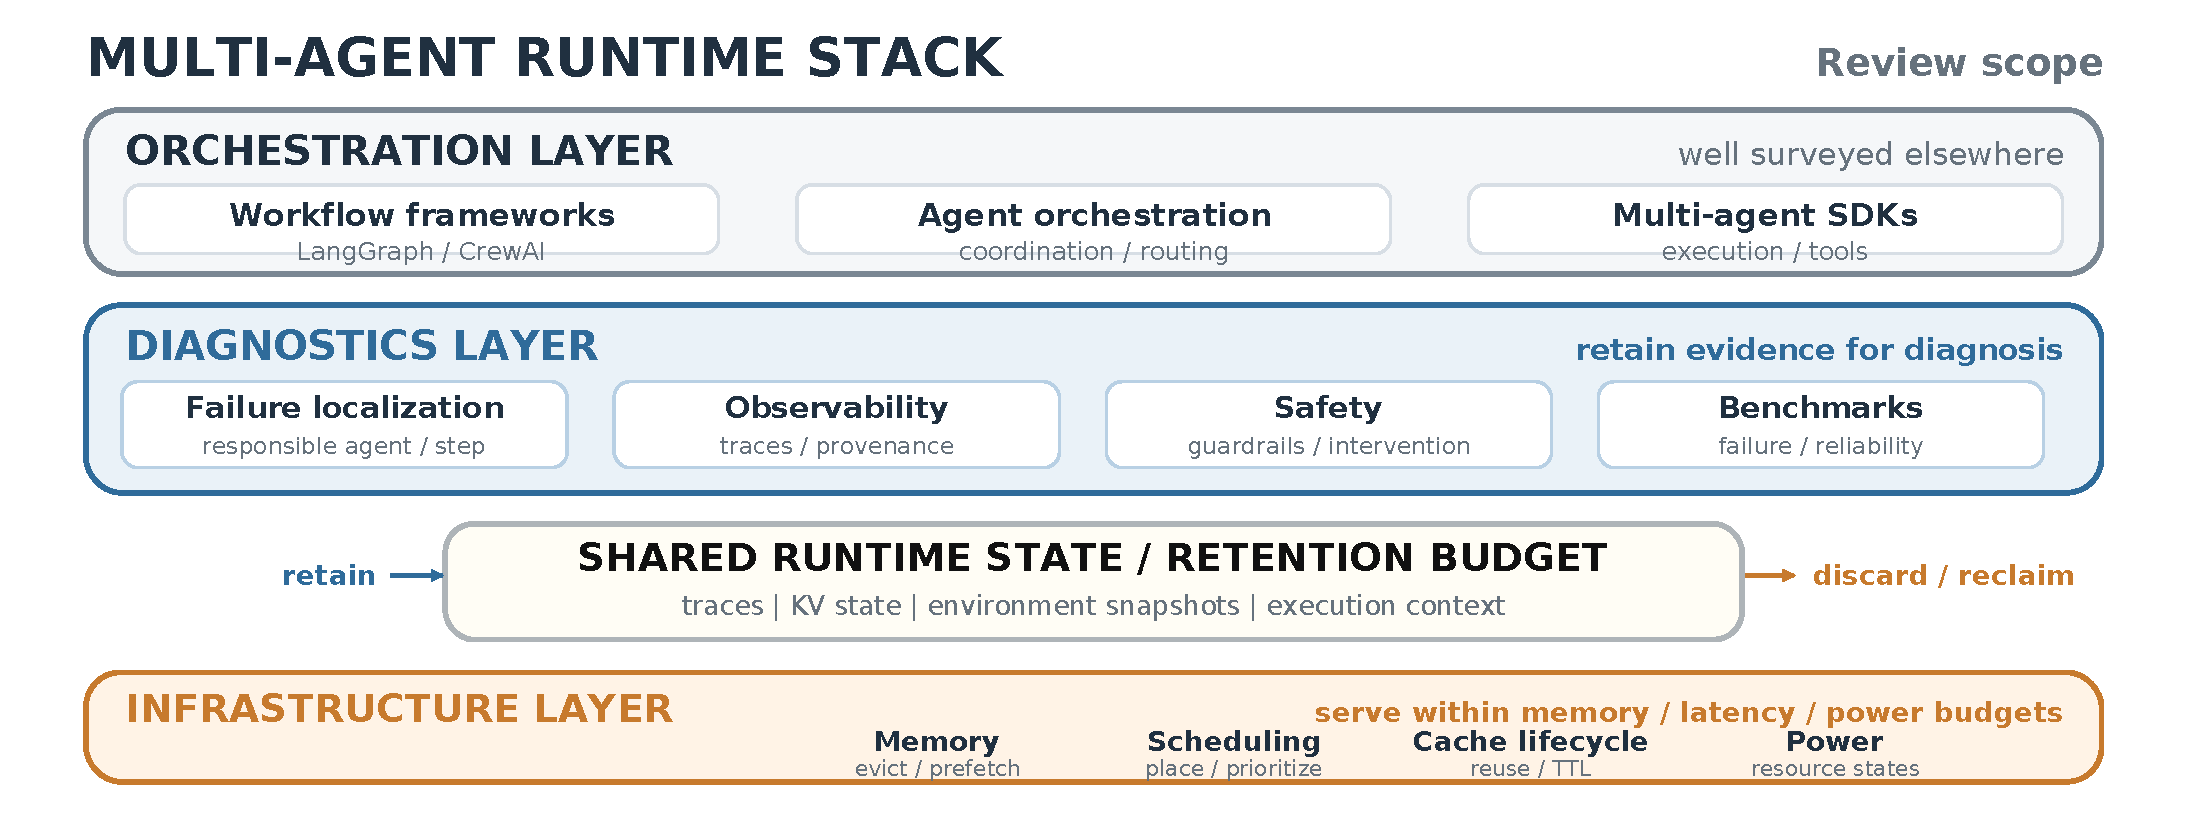
\includegraphics[width=\textwidth]{fig1_overview.pdf}
\caption{Survey scope: the multi-agent runtime stack. Our survey covers the diagnostics layer (\S\ref{sec:diagnostics}) and the infrastructure layer (\S\ref{sec:infrastructure}); the orchestration layer (top, dashed) is well-covered by existing surveys. The two-way arrow marks the retention tension analyzed in \S\ref{sec:tension}, which connects the two layers.}
\label{fig:overview}
\end{figure*}

Our contributions are:
\begin{enumerate}
\item \textbf{Diagnostics taxonomy.} We organize multi-agent diagnostics into four subcategories spanning failure localization (\S\ref{sec:diag_fl}), observability (\S\ref{sec:diag_obs}), safety (\S\ref{sec:diag_safety}), and benchmarks (\S\ref{sec:diag_bench}), covering three failure localization paradigms (statistical, LLM-guided, RL-trained) and three safety paradigms (topology-based, policy verification, ML-layered).
\item \textbf{Infrastructure challenge analysis.} We identify three multi-agent workload characteristics (sparse activation, invocation distance, inter-agent memory sharing) that existing single-LLM serving systems do not exploit predictively, demonstrated through application-aware systems spanning memory optimization (ScaleSim, up to 1.74$\times$ speedup~\citep{zhou2026}), prefix-aware scheduling (TokenCake~\citep{tokencake2025}), cache lifecycle (Continuum), and power management (KAIROS).
\item \textbf{Cross-layer tension analysis.} We identify and analyze the fundamental conflict between the two layers, namely that diagnostics must \emph{retain} runtime state while serving infrastructure must \emph{discard} it, and derive four co-design opportunities from this tension rather than listing them in isolation (\S\ref{sec:tension}, with the opportunities developed in \S\ref{sec:discussion}).
\end{enumerate}